\documentclass[a4paper, 12pt]{article}

\usepackage{amsmath}
\usepackage{amssymb}
\usepackage{parskip}
\usepackage{hyperref}
\usepackage{graphicx}
\usepackage{xcolor}
\usepackage{tcolorbox}
\usepackage{fullpage}
\usepackage{tikz}
\usepackage{changepage}
\usepackage{framed}
\usepackage[sorting=none]{biblatex}
\usepackage{csquotes}
\usepackage[italian]{babel}
\usepackage{eso-pic}
\usepackage{stackengine}
\usepackage{adjustbox}
\usepackage{emoji}

\usetikzlibrary{arrows,positioning}

\graphicspath{ {./images/} }

\newcommand{\quotes}[1]{``#1''}

\newcommand\BackgroundPic{
    \put(0,0){
        \parbox[b][\paperheight]{\paperwidth}{
            \vfill
            \centering
            
\includegraphics[width=\paperwidth,height=\paperheight]{background}
            \vfill
        }
    }
}

\newcommand{\ownright}[0]{% don't remove
    \makebox(0,0){
        \stackon[8pt]{\phantom{A}}{
            \begin{tikzpicture}
                \fill (0,0) -- (0,0.3) -- ++(0.05,0) -- (0.05,0);
                \fill (0,0.3) -- ++(0.3,0) -- (0.3,0.25) -- (0.05,0.25);
            \end{tikzpicture}
        }
    }%
}

\newcommand{\ownleft}[0]{% don't remove
    \makebox(0,0){
        \stackon[-8pt]{\phantom{A}}{
            \begin{tikzpicture}
                \fill (0,0) -- (0.3,0) -- ++(0,0.05) -- (0,0.05);
                \fill (0.3,0) -- ++(0,0.3) -- (0.25,0.3) -- (0.25,0.05);
            \end{tikzpicture}
        }
    }
}

\hypersetup{
    colorlinks=true,
    linkcolor=black,
    urlcolor=blue,
    pdftitle={Paolo Bettelini - PDI},
    pdfpagemode=FullScreen,
}

\addbibresource{references.bib}

\title{
    \textsc{Il ruolo dello Stato democratico nella società umana}
    \\
    {\small \textsc{La moralità del sistema giudiziario}}
}

\author{
    \textsc{Paolo Bettelini}
    \\
    \textsc{\large Scuola d'Arti e Mestieri di Trevano (SAMT)}
}

\date{\textsc{\today}}

\linespread{1.25}

\begin{document}

\AddToShipoutPicture*{\BackgroundPic}

\makeatletter
\renewcommand{\maketitle}{
    \vspace*{20pt}
    \begin{adjustwidth}{}{-1in}
        \begin{flushright}
            \begin{tcolorbox}[sharp corners,
                colback=white,
                colframe=white,
                text width=\dimexpr9cm+1in]
                
                \centering
                
                {\LARGE\@title}
                
                \vspace{30pt}
                
                {\large\@author}
                
                \@date
                
                \vspace{20pt}
            \end{tcolorbox}
        \end{flushright}
    \end{adjustwidth}

    \vspace{10cm}

    \begin{adjustwidth}{-1in}{}
        \begin{flushleft}
            \begin{tcolorbox}[sharp corners,
                colback=white,
                colframe=white,
                text width=\dimexpr5cm+1in]
                
                Progetto Didattico Interdisciplinare
                
                Classe I4AC 2022/2023 | PDI
                
                Monica Delucchi, Ursula Holliger
            \end{tcolorbox}
        \end{flushleft}
    \end{adjustwidth}
}
\makeatother

\maketitle

\pagebreak

\tableofcontents
\pagebreak

\section{Introduzione}

\subsection{Il progetto didattico interdisciplinare}

Il progetto didattico interdisciplinare (PDI) è un lavoro originale e personale
con un tema. Il tema generale è \quotes{Il ruolo dello Stato democratico nella società umana}.
Ho scelto di affrontare questo tema parlando della moralità del sistema giudiziario,
una parte fondamentale di ogni democrazia. \\
Questo testo prova a rispondere alla domanda \quotes{\textit{quanto è morale il sistema giudiziario?}}.

\subsection{Biografia}

Durante la mia vita mi sono ritrovato a sviluppare dei pensieri
spesso in discordia con la maggior parte delle persone.
Mediante delle successioni di pensieri logici, ho scoperto autonomamente concetti
come il \textit{determinismo}, senza aver mai avuto nessun contatto con dei testi di filosofia.
\\
Questo lavoro è una riflessione personale che sviluppa i miei pensieri
personali circa la moralità delle cose. Verranno trattate le implicazioni
che questi concetti hanno sulla democrazia e sul sistema giudiziario.

Il documento tratterà la democrazia semplicemente come il concetto di integrare i cittadini
nel governo di una società. Non verranno discussi i diversi modelli di democrazia o di stato
poiché non strettamente attinenti all'argomento.

Le prime sezioni del documento introducono quelli che sono i concetti fondamentali per
sviluppare il mio ragionamento. In seguito verranno trattate
le implicazioni di questi concetti sulla moralità di uno stato e come si potrebbero
ipoteticamente risolvere.

\subsection{Il mio pensiero}

Il mio pensiero consiste in una riflessione circa la moralità delle pene.
Date una serie di affermazioni sulla natura dell'universo, ritengo che l'essere umano
non possegga il libero arbitrio. Questa assenza priva di significato alcuni concetti come la
\textit{pena} o il \textit{merito}. Sostanzialmente, ritengo che sia immorale punire gli esseri
umani per le loro azioni. Ciò non implica che un criminale non debba essere allontanato dalla società,
in quanto un pericolo, un provvedimento va comunque effettuato. Tuttavia,
il fatto stesso di punire una persona è intrinsicamente immorale per via
della sua impossibilità di non commettere le azioni che ha commesso.

\pagebreak

\subsection{Struttura}

La struttura di questo lavoro può essere rappresentata con il seguente diagramma.

\vspace{0.75cm}

\tikzset{
    %Define standard arrow tip
    >=stealth',
    %Define style for boxes
    important/.style={
           rectangle,
           rounded corners,
           draw=black, very thick,
           text width=6.5em,
           minimum height=2em,
           text centered},
    % Define arrow style
    pil/.style={
           thick,
           shorten <=2pt,
           shorten >=2pt,}
}

\begin{figure}[h]
    \centering
    \begin{tikzpicture}[node distance=1cm, auto]
        \node[important] (demo) {Democrazia};

        \node[below=of demo] (sg) {Sistema Giudiziario}
            edge[pil, <-] (demo);

        \node[below=of sg] (center1) {};

        \node[right=of center1] (mor) {Moralità};
        \node[below=of center1] (pene) {Pene};
        \node[left=of center1] (soc) {Società};

        \path (sg.east) edge[->, pil, bend left=30] (mor);
        \path (mor) edge[->, pil, bend left=30] (pene.east);
        \path (pene.west) edge[->, pil, bend left=30] (soc);
        \path (soc) edge[->, pil, bend left=30] (sg.west);
        
        \node[right=of mor] (lib) {\underline{Libero arbitrio}}
            edge[pil, <-] (mor.east);

        \node[right=of lib] (center2) {};

        \node[above=of center2] (det) {Determinismo};
        \node[below=of center2] (cas) {Casualità};

        \path (lib) edge[->, pil, bend left=45] (det.west);
        \path (lib) edge[<-, pil, bend right=45] (cas.west);
        \path (det.east) edge[->, pil, bend left=45] (cas.east);

        \node[below=of pene] {Cenni Storici}
            edge[pil, <-] (pene);
    \end{tikzpicture}
    \caption{Struttura del documento}
\end{figure}

Il sistema giudiziario è una parte fondamentale di ogni
sistema giuridico e democrazia.
Questo lavoro analizza la moralità delle pene
imposte dal sistema giudiziario da un punto di vista filosofico.
A questo scopo vengono analizzate alcune correnti di pensiero come il determinismo.
Gli strumenti utilizzati per studiare il determinismo
hanno fondamenta nella fisica. Questi argomenti sono
apparentemente fuori tema, tuttavia, sono necessari
per affrontare le argomentazioni filosofiche e per cui strettamente
legate allo scopo di questo testo.

\vspace{4cm}

\textbf{Nota}:
\begin{enumerate}
    \item I blocchi di testo racchiusi con \hspace{0.2cm}\ownright{}\quotes{}\ownleft{}
    \hspace{0.2cm} esprimono dei concetti, ragionamenti o idee che sono stati puramente sviluppati da me.
    \item Il documento presenta delle definizioni di termini reali o fabbricati solamente per lo scopo di
        questo scritto, denominate con \textbf{Def. \quotes{}}.
\end{enumerate}

\pagebreak

\section{Etica e Morale}

\subsection{Definizione}

\paragraph{Def. Morale:}
la morale è un insieme di pensieri, decisioni e comportamenti che secondo l'individuo
che li esercita sono \textit{corretti} nei confronti di sé stesso o di terze parti.

\paragraph{Def. Etica:}
L'etica è un insieme di pratiche, comportamenti e di norme che vengono applicati
per rispecchiare un'ideologia morale collettiva.

La moralità è certamente soggettiva ed è estremamente
difficile esporne un'accezione in maniera oggettiva.

\subsection{Il regno animale}

Seppur molti animali mostrino comportamenti empatici e molte emozioni umane,
molte specie commettono azioni che potrebbero essere giudicate come spregevoli da noi umani.
Senza considerare il bisogno naturale del cacciatore di uccidere, talvolta in maniera brutale,
la preda per sopravvivere, le azioni che noi potremmo ritenere immorali
riguardando anche l'ambito sociale fra gli animali e quello sessuale.
Per esempio, alcune specie di pinguini sono stati osservati praticare
pedofilia, necrofilia, stupro e addirittura stupro di altri pinguini soccombenti
\cite{penguins}.

Gli animali dimostrano comunque comportamenti guidati da principi morali
\cite{rowlands2012oxford} \cite{rowlands2015can} \cite{andrews2018routledge}.
Possono infatti mostrare comportamenti che potrebbero essere considerati morali dal punto di vista umano,
come prendersi cura dei loro piccoli o aiutare i loro simili in difficoltà.

\section{Il libero arbitrio}

Il libero arbitrio è un concetto per il quale gli esseri umani
(o, in alcune eccezioni, ogni essere cosciente) sono in grado di decidere e agire secondo la propria volontà.
L'essere è quindi libero di arbitrare le proprie azioni secondo la sua volontà.
Molte filosofie e teorie religiose credono infatti che l'essere umano sia in grado
di scegliere il proprio destino secondo il proprio arbitrio.

\pagebreak

\section{Il determinismo}

\subsection{Definizione}

Il determinismo\cite{det} è una corrente di pensiero che esprime l'idea
che gli eventi dell'universo siano completamente determinati e prevedibili.
\\
Vi sono diverse versioni di questo pensiero e
molti filosofi hanno sviluppato i concetti, fra cui Platone, Kant,
Nietzsche e Confucio.

\subsubsection{Determinismo assoluto}

Il determinismo assoluto è la versione più severa del determinismo.
Questo pensiero indica che tutti gli eventi siano strettamente
determinabili dagli eventi dell'universo precedenti.
Conoscendo l'esatto stato dell'universo in un dato istante \(t_n\), è possibile
determinare un qualsiasi istante futuro \(t_{m > n}\).
Questo implica anche che tutto il futuro dell'universo sia,
in un certo senso, predeterminato, dal momento che ogni evento è destinato
a succedere in una certa maniera.

Questo ideologia è in contrapposizione con il libero arbitrio.
Dal momento che tutti gli eventi nell'universo sono determinati da altri fattori determinati
o determinabili, i processi biologici che ci permettono di prendere delle decisioni e di pensare
sono soggette al determinismo assoluto, in quanto facenti parti di un sistema fisico esistente nell'universo.

\subsubsection{Compatibilismo}

Il compatibilismo\cite{com} è una corrente di pensiero che prevede una compatibilità
fra il libero arbitrio ed il determinismo. Un'accezione generica di questa ideologia
implica che l'uomo abbia infatti il potere di scegliere liberamente secondo la sua volontà.
Tuttavia, questa teoria è molto criticata e molte persone credono che
il libero arbitrio e il determinismo siano concetti inconciliabili.
Il concetto che l'essere umano abbia la capacità di scegliere liberamente le proprie azioni,
ma queste scelte siano comunque determinate da cause esterne,
come le proprie inclinazioni, le proprie esperienze e le proprie circostanze,
è fondamentalmente contrario al determinismo.
Esiste anche un'accezione del compatibilismo in cui le azioni sono
esenti dai fenomeni deterministici in quanto strettamente legate alla coscienza o all'anima.
Questa accezione implica l'esistenza di una proprietà non tangibile
appartenenti agli essereri viventi, l'anima, la quale permetterebbe di compiere
azioni puramente dettate dal proprio io spirituale.

\subsection{Determinismo nella fisica}

Il mondo in cui viviamo è governato dalla meccanica.
Tutte le nostre azioni quotidiane sono governate dalla meccanica.
Guidare l'auto, fare cadere un oggetto, camminare etc. sono tutte azioni
che rispettano delle leggi fisiche ben conosciute. \\
Agli inizi del XX secolo la comunità scientifica ha cominciato ad esplorare ciò che
oggi viene chiamata la meccanica quantistica. Queste nuovi leggi secondo le quali il nostro universo funziona
ad un livello microscopico, hanno generato diverse critiche verso il determinismo.
Queste leggi potrebbero infatti indicare che l'universo non si basa unicamente su eventi deterministici ma anche eventi casuali.

\subsubsection{Principio di indeterminazione di Heisenberg}

Il principio di indeterminazione di Heisenberg è molto importante nelle discussioni
legate al determinismo e alla natura intrinseca dell'universo.
Questo principio fisico indica infatti che, considerando un oggetto quantistico (di dimensioni molto piccole),
l'ammontare di conoscenza sulla sua velocità è inversamente proporzionale all'ammontare
di conoscenza sulla sua posizione.
Se conosciamo esattamente la posizione di un oggetto, non sappiamo nulla sulla sua velocità.
Se conosciamo esattamente la sua velocità, non sappiamo nulla sulla posizione. Se siamo un po'
incerti sulla sua velocità, siamo anche un po' incerti sulla sua posizione.
La nostra conoscenza \textit{simultanea} di alcune proprietà è vincolata da delle leggi fisiche. \\
Questa affermazione può sembrare assurda e priva di senso, ma nel campo quantistico
alcune proprietà sono descritte da delle probabilità piuttosto che da dei valori sempre concreti.

Considerando questo fenomeno fisico possiamo giungere ad una contraddizione nel determinismo.
Non è possibile conoscere lo stato dell'universo ad un certo istante se non possiamo
conoscere simultaneamente tutte le proprietà del nostro sistema.
Alcune proprietà sono intrinsecamente \textit{incerte}, per cui
dettate da un sistema probabilistico. Questo vincolo implica che
le azioni appartenenti ad un istante futuro \(t_m\) rispetto ad un istante
\(t_{n < m}\) non sono determinabili in quanto dettati da eventi probabilistici
e non solo semplici successioni di avvenimenti.

\subsubsection{Eventi casuali}

La fisica quantistica è governata da funzioni probabilistiche.
Una funzione probabilistica è una funzione che descrive un fenomeno. Essa
esprime la possibilità che ogni possibile risultato avvenga. Per esempio,
una funzione probabilistica potrebbe descrivere l'altezza delle persone.
Scegliendo una persona qualsiasi in una piazza, abbiamo un'alta probabilità che la sua altezza
sia all'incirca 170cm, mentre abbiamo una probabilità più bassa che la persona sia alta 150cm oppure 190cm.
Questo è ciò che descrive una funzione di questo tipo, notiamo come ogni persona abbia il 100\% di probabilità
di avere un'altezza (la funzione descrive tutti i possibili risultati).
Per quel che concerne la meccanica quantistica basti pensare alla posizione di un elettrone. La posizione di un elettrone
di un sistema può essere descritta da una \textit{funzione d'onda}. Questa funzione descrive
la probabilità di misurare l'elettrone in un certo punto. Per esempio, considerando un elettrone libero
di trovarsi su una linea, potrebbe essere molto probabile che esso venga misurato essere nello spazio centrale, mentre
poco probabile che si trovi agli estremi.

\begin{figure}[h]
    \centering
    \begin{tikzpicture}
        \draw[domain=-2:2, smooth, variable=\x, blue, very thick] plot ({\x}, {2.718^(-1*\x*\x)});
    
        \draw[->] (0, -0.25) -- (0, 1.25) node[above] {\(|\Psi(x,t)|^2\)};
        \draw[->] (-2.25, 0) -- (2.25, 0);
    \end{tikzpicture}
    %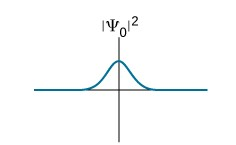
\includegraphics[width=0.5\textwidth]{wavefunction.jpg}
    \caption{Funzione d'onda}
\end{figure}

La natura deterministica dell'universo è dunque strettamente legata all'esistenza di
eventi puramente casuali.

\paragraph{Def. Evento pseudo-casuale:} Un evento pseudo-casuale o un numero pseudo-casuale è un evento
che approssima una probabilità ma è in realtà deterministico.
Il lancio di un dado o di una moneta sono degli eventi pseudo-casuali.
La probabilità che una moneta atterri in una certa maniera è 50\%, tuttavia,
questo risultato è ben definito dalle leggi fisiche della meccanica. \\
Un altro esempio sono i numeri randomici generati dai computer, essi sono infatti
pseudo-casuali. Il computer sfrutta il numero di millisecondi passati dall'1 gennaio 1970 (unix-time).
Questo valore è molto volatile e per cui ottimale per generare una distribuzione
omogenea di numeri casuali. \\
Ci sono molti valori volatili in natura. Misurare la temperatura con un termometro
e considerare alcune cifre dalla decima cifra in poi dopo la virgola risulta
in un numero quasi casuale.
Tutti questi fenomeni possono essere ricostruiti date le condizioni di partenza.

\paragraph{\ownright{}Def. Evento puramente casuale:} Un evento puramente casuale
è un qualsiasi evento che potrebbe svolgersi in maniera differente se l'universo venisse riavvolto per ripetere nuovamente tale evento, senza che l'esecuzione dell'evento a priori abbia alcun effetto sulla nuova esecuzione.

Se nell'universo sono presenti eventi puramente casuali il determinismo non è corretto
in quanto non tutti gli avvenimento sono deducibili dagli eventi precedenti.

Gli eventi casuali presenti nella meccanica quantistica sono puramente casuali
oppure possono essere deducibili da altri fattori (pseudo-casuali)?
Questa è la domanda saliente circa il determinismo.
Se gli eventi puramente casuali dovessero esistere l'universo non si potrebbe basare unicamente
su regole deterministiche.
La scienza non è mai riuscita a dimostrare o sfatare nessuna delle due ipotesi.

Spesso il termine \quotes{evento casuale} o \quotes{numero casuale} viene utilizzato
in contrapposizione a \quotes{numero pseudo-casuale}.
Solitamente non vi è distinzione fra la mia definizione di \textit{evento puramente casuale}
e quella di un evento casuale descritto da una funzione probabilistica.
Per questo testo tutti i fenomeni vengono classificati in due categorie:
quelli puramente casuali e tutti gli altri.%
\ownleft{}

\subsection{Determinismo nell'anatomia}

La seguente sezione tratta in maniera generale il funzionamento del cervello
e come prendiamo ogni decisione.

Il cervello è una macchina molto complessa che nessuno
comprende pienamente. Tuttavia, la scienza riesce a spiegare a grandi linee
il sistema decisionale. Questo sistema si basa su tante piccole strutture cellulari
facenti parti del sistema neuroso, i \textit{neuroni}.

\begin{figure}[ht]
    \centering
    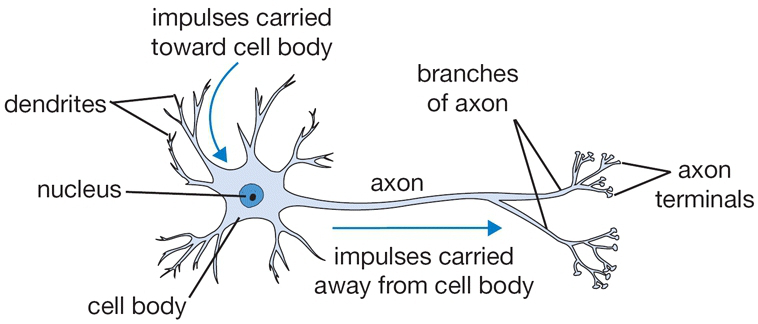
\includegraphics[width=0.75\textwidth]{neuron.png}
    \caption{Struttura neuronale}
\end{figure}

I neuroni\cite{neuron} sono a loro volta composti da diversi elementi.
I dendriti sono delle estensioni sottili e ramificate che ricevono segnali elettrici da altri neuroni.
Il nucleo è un organello presente nel corpo cellulare di un neurone.
Contiene il materiale genetico della cellula e ne controlla il metabolismo e
altre funzioni.
L'assone è un'estensione lunga e sottile di un neurone che conduce gli impulsi elettrici
lontano dal corpo cellulare.
Il corpo cellulare è la parte centrale di un neurone che contiene
il nucleo cellulare e altri organelli.
Le terminazioni assoniche sono piccole strutture alla fine di un assone che trasmettono
segnali ad altre cellule. La zone di connessione
fra due neuroni viene chiamata \textit{sinapsi}.

Sostanzialmente, un neurone invia un impulso ad altri neuroni
a seconda degli impulsi elettrici che riceve.
Questa topologia è in costante cambiamento. Infatti,
nuove connessioni fra neuroni sono sempre stabilite.
L'insieme dei funzionamenti di tutti questi organi permettono al nostro
corpo di prendere qualsiasi decisione.

\ownright{}%
\textbf{Def. I 3 fattori:} Possiamo dunque dedurre che ogni decisione mai presa da ognuno di noi è
sostanzialmente dipendente da 3 fattori:
\begin{enumerate}
    \item Configurazione genetica iniziale
    \item Eventi vissuti
    \item Ambiente circostante
\end{enumerate}

\paragraph{Configurazione genetica iniziale}
Il modo di pensare è diverso fra persona e persona.
Uno dei fattori molto importanti è la configurazione anatomica iniziale del cervello,
ossia la configurazione iniziale di sinapsi, neuroni etc. alla nascita.

\paragraph{Eventi vissuti}
Ogni evento vissuto può modificare la nostra capacità di pensare.
Un evento può consistere in un'interazione fisica o semplicemente qualcosa di visto.
Durante la vita le configurazioni delle sinapsi evolve costantemente. Provare certe esperienze
o trovarsi in certe situazioni può certamente alterare la nostra capacità cognitiva.
Un evento può per esempio consistere nell'alterazione fisica del cervello, come per esempio
un intervento di leucotomia oppure la malattia del morbo di Alzheimer.

\paragraph{Ambiente circostante}
Al momento di prendere una decisione l'ambiente circostante è uno dei principali fattori
principali. A seconda della situazioni, cerchiamo di prendere una decisione auspicabile
per affrontare quest'ultima.%
\ownleft{}

\pagebreak

\subsection{Implicazioni nella moralità}

Assumendo il determinismo si giunge ad un concetto che può essere molto pericoloso per una società
e le persone stesse. Questo concetto è la perdita del significato della colpa o della responsabilità, del merito e altri simili.

\ownright{}%
Dal momento che ogni scelta presa
da un uomo è determinata da 3 fattori e
quest'ultimi sono deterministici, possiamo
dedurre che tutte le scelte sono
anch'esse deterministiche.
Ogni uomo è, in un certo senso, destinato a
svolgere qualsiasi azione nella sua vita.
L'uomo non è intrinsecamente responsabile
per le sue azioni. Nessuno ha veramente colpa di qualcosa oppure
merito. Nessuno è malvagio o buono. Questo
implica anche che tutte le azioni umane siano
neutrali secondo la natura dell'universo.

Questo universo, dove assumiamo il determinismo, può essere considerato come un gioco del domino in un universo deterministico.
Ogni caduta di una tessera è causata dalla caduta di quelle precedenti. Ogni azione è determinata da quelle precedenti
e, riposizionando le tessere con la medesima configurazione
iniziale, si otterrà lo stesso risultato.
In maniera equivalente qualsiasi cosa in un 
universo deterministico è come una tessera che cade
e ne spinge un'altra. Questo comprende anche i nostri
pensieri e comportamenti.

Dobbiamo comunque considerare anche il caso in cui
il nostro universo non fosse deterministico, bensì
caratterizzato anche da eventi puramente casuali.
Così facendo consideriamo estensivamente ogni possibilità
della natura dell'universo, dal momento che
l'universo contiene eventi puramente casuali oppure
non li contiene.

Assumendo la presenza di eventi puramente casuali,
l'analogia del domino cambia leggermente.
Il gioco del domino adesso si svolge in un universo
dove esistono eventi puramente casuali a livello microscopico.
Questi eventi potrebbero alterare leggermente
le traiettorie delle tessere in maniera casuali.
Queste piccole imperfezioni fanno sì che,
riposizionando le tessere con la configurazione iniziale,
il risultato potrebbe essere leggermente diverso
secondo un fattore casuale. Tuttavia,
la caduta delle tessere è prevalentemente
causata dalla caduta di quelle precedenti.
Ogni avvenumenti non è solamente dettato da quelli precedenti
ma anche in parte da una fattore randomico.

In un universo di questa tipologia, le azioni umane
sono sempre determinate dai 3 fattori.
Questi fattori presentano tuttavia una piccola
parte derivante da eventi casuali.
Questa tipologia di universo è comunque un gioco
del domino.

Possiamo quindi dedurre che, indipendentemente dal fatto
che l'universo sia deterministico o meno
per quel che riguarda gli eventi puramente casuali,
tutte le azioni sono neutre e gli umani compiono
ogni decisione in maniera passiva, senza libero arbitrio.%
\ownleft{}

\pagebreak

\section{Il sistema giudiziario}

\subsection{Definizione e democrazia}

Il sistema giudiziario è il meccanismo attraverso il quale il sistema giuridico
viene applicato e fatto rispettare.
Include i tribunali e gli altri organismi che sono responsabili
dell'applicazione delle leggi e della risoluzione delle controversie legali.
Il sistema giudiziario è formato da giudici, avvocati e altri
che lavorano per risolvere le controversie legali in modo equo e giusto.
In sostanza il sistema giudiziario si occupa di condannare gli atti illeciti
al fine di mantenere il quieto vivere.

\subsection{Cenni storici}

\subsubsection{La legge del taglione}

La legge del taglione\cite{taglione} è un principio giuridico secondo il quale una persona
che ha subito un torto ha il diritto di riparare il danno subito
con un'azione simile a quella subita verso il responsabile del torto.
Questa legge deriva dalla tradizione giuridica ebraica e viene spesso citata nella Bibbia.
La legge del taglione è stata utilizzata in diverse culture e sistemi giuridici
nel corso della storia, oggi non è più riconosciuta come un principio legale valido
in molti paesi.
Alcuni concetti legati alla legge del taglione
sono ancora presenti nei sistemi giuridici odierni,
come il principio della \quotes{pena adeguata} per un reato commesso.

\subsubsection{La ghigliottina}

La ghigliottina\cite{ghigliottina} è un simbolo molto importante per quel che riguarda
la storia delle pene.
Questo strumento veniva utilizzato per le esecuzione in alcuni paesi europei,
tra cui Francia, Belgio e Italia, fino alla metà del XX secolo.
Consisteva in una macchina costituita da una lama
verticale che scendeva in modo rapido e preciso per recidere il
collo della persona condannata a morte.

La ghigliottina era spesso utilizzata come mezzo di esecuzione pubblica
e la sua introduzione era stata giustificata come un modo di rendere più umana
e meno crudele l'esecuzione, poiché si sosteneva che la lama affilata
avrebbe causato una morte rapida e indolore.
Alcuni studi hanno suggerito che le persone giustiziate con la
ghigliottina potrebbero aver sofferto dolore durante l'esecuzione
a causa della lesione dei nervi.

La ghigliottina è stata utilizzata per la prima volta in Francia durante la Rivoluzione francese
nel 1792 e rimase in uso fino alla fine degli anni '70,
quando l'ultima esecuzione con la ghigliottina ebbe luogo in Francia nel 1977.
Oggi, la pena di morte è stata abolita in molti paesi e la ghigliottina non viene più
utilizzata come mezzo di esecuzione \cite{ghigliottina}.

\subsubsection{Cesare Beccaria}

Cesare Beccaria\cite{cesare} (1738-1794) è stato un giurista e filosofo italiano.
Nel 1764 pubblica \quotes{Dei delitti e delle pene} (cita) 
dove esamina una serie di difetti nel sistema dell'epoca che imponevano una giustizia equa.
Questa'opera è molto importante poiché delimita il peccatto (peccato religioso
che viene giudicato da Dio) da ciò che bisogna considerare da un punto di vista giuridico,
applicando leggi eque e uguali per tutti.

Cesare Beccaria era contrario alla pena di morte e alla tortura, infatti,
voleva dimostrare che queste metodologie fossero inefficaci e disumani.
Una delle sue idee primarie era l'importanza di prevenire un delitto piuttosto che punirlo.

Beccaria era convinto che il sistema penale del suo tempo fosse iniquo e crudele,
e che fosse necessario riformarlo per rendere le pene più umane e proporzionate ai reati commessi.
Nel suo libro, Beccaria affermava che l'obiettivo principale delle pene non doveva essere la vendetta,
ma la prevenzione dei reati stessi, specialmente mediante l'educazione dei cittadini.
Le sue idee hanno influenzato profondamente il pensiero giuridico e politico dell'epoca
e hanno contribuito ai principi della rivoluzione francese e alla nascita delle moderne
costituzioni democratiche.

\subsection{Moralità nel sistema giudiziario}

Dati i ragionamenti logici nelle sezioni precedenti, è morale punire
un criminale?

\textbf{Def. Sanzione riparatoria:} Le sanzioni riparatorie hanno
lo scopo di riparare il danno causato da una violazione
o di impedire che si verifichino ulteriori violazioni.
Ad esempio, se una persona commette un reato ambientale,
potrebbe essere obbligata a svolgere servizi socialmente utili
o a pagare una somma di denaro per coprire i costi della riparazione del danno.

\textbf{Def. Sanzione punitiva:} Le sanzioni punitive,
al contrario, hanno lo scopo di punire il colpevole
per la violazione commessa e di dissuadere altre persone
dal commettere violazioni simili in futuro.
Ad esempio, una persona che commette un reato potrebbe essere condannata
a una pena detentiva o a un'ammenda.

\enquote{
Secondo il principio della \textit{finalità rieducativa della pena}, le pene
non devono essere volte unicamente alla punizione del reo ma
devono innanzitutto mirare alla sua rieducazione,
quale requisito fondamentale per il suo reinserimento nella società.
}\cite{rieducazione}.

\ownright{}%
Una persona che ha commesso un crimine ed è nefasta
nei confronti della popolazione deve certamente essere allontana dalla società.
Tuttavia, considerando i ragionamenti svolti circa le azioni umane,
è immorale punire un criminale dal momento che non avrebbe potuto evitare di commettere
le azioni commesse.

Possiamo giungere alla medesima conclusione senza parlare
dell'aspetto filosofico della natura dell'universo, bensì mediante un'analogia.

\textbf{Def. Deviazione:} Con il termine deviazione voglio intendere
un qualsiasi deviamento da un essere umano che funziona perfettamente,
sia a livello fisico che a livello sociale. Questo può comprendere
qualsiasi malattia, fisica o mentale, virus, difetto genetico,
difetto indotto etc.

Supponiamo che un uomo abbia una insufficienza epatica.
Sarebbe totalmente assurdo e illogico se quest'uomo dovesse venir
punito per il solo motivo di avere un problema al fegato.
Supponiamo ora che un uomo commetta commetta una sparatoria in una scuola.
In questo caso la punizione dell'uomo sembra molto più razionale e corretta.
Possiamo considerare questo comportamento come un disturbo mentale, in altre parole,
una deviazione.

Un problema al fegato ed un disturbo mentale del genere sono due cose molto diverse.
L'unica similitudine fra le due cose è il fatto che sono entrambe delle deviazioni.
Entrambe le supposizioni implicano che un organo non stia funzionando
nella maniera corretta, nel primo caso, il fegato, mentre nel secondo, il cervello.
C'è una grossa distinzione fra la prima supposizione e la seconda, e per esporla
faremo un terzo scenario contenente un'altra deviazione: \\
Supponiamo che un uomo contragga la malattia da virus Ebola.
Questo terzo scenario è molto più vicino al secondo scenario di quanto
non lo sia il primo, in quanto in questo caso, la persona con la deviazione
è un pericolo per le persone con cui entra in contatto. Questa persona
va isolata in maniera tale da evitare di fare del male ad altri individui.
Possiamo quindi fare la seguente distinzione \\
\textbf{Def. Deviazione di tipo 1:} Una deviazione che non può nuocere altre persone. \\
\textbf{Def. Deviazione di tipo 2:} Una deviazione che può mettere in pericolo altre persone.

Punire una persona per una deviazione di tipo 1 sarebbe assolutamente
immorale.
Punire una persona per una sua deviazione è immorale dal momento
che ogni organo potrebbe smettere di funzionare nella maniera corretta.
Nel caso di una deviazione di tipo 2 è tuttavia necessario allontanare il
soggetto dal resto della società.%
\ownleft{}

\pagebreak

\subsection{Implementazione alternativa}

\ownright{}%
Partendo dal presupposto che punire un criminale sia immorale,
come si potrebbe aggiunstare di conseguenza il sistema giudiziario?

Dare una risposta coincisa a questa domanda è estremamente complesso.
Considerare questo valore morale nel quadro generale
ha solamente svantaggi e nemmeno un vantaggio funzionale:
\begin{enumerate}
    \item Perdita del deterrente: le pene sono sempre state
        un deterrente per evitare che altri cittadini commettessero
        crimini. Se un cittadino non viene punito dopo aver commesso
        un reato è probabile che molti cittadini commettano più crimini.
    \item Perdita del valore della colpa: considerando
        i ragionamenti logici effettuati sulla natura delle azioni umani
        e sul libero arbitrio, la perdita del valore della colpa potrebbe
        spingere i cittadini a commettere più crimini.
        Questo creerebbe una sorta di ideologia nichilista
        dove le persone agiscono senza conseguenza, rendendo
        impossibile il quieto vivere.
\end{enumerate}

Un'implementazione alternativa dovrebbe concentrarsi unicamente
allo scopo riparativo piuttosto che punitivo.
In un eventuale futuro, potrebbe essere possibile utilizzare la
tecnologia per rieducare gli individui. In questo scenario
ci sarebbero comunque dei problemi, per esempio,
bisognerebbe evitare di violare la libertà dell'individuo stesso,
nel caso in cui non volesse essere rieducato.

In conclusione, ritengo personalmente che l'atto di infliggere
una sanzione punitiva su un criminale sia immorale da un punto di vista
prettamente filosofico. Tuttavia, aggiustare di conseguenza
il sistema giudiziario odierno sarebbe quasi impossibile
e non auspicabile.%
\ownleft{}

\pagebreak

\section{Conclusione e considerazioni}

\ownright{}%
Sono molto felice di avere avuto la possibilità di lavorare su questo tema.
Per la maggior parte della mia vita ho sempre avuto pensieri circa
questi argomenti, e finalmente ho trovato l'opportunità per scriverne al riguardo.
Il tema è molto complesso ma soprattutto sensibile.
Le mie idee possono apparentemente sembrare incitanti all'odio e al crimine,
tuttavia, sono totalmente contrario a tutto ciò.

Mi sono accorto che moltissime persone nutrono un odio spropositato
verso i criminali. In particolare, pedofili o chiunque commetta
crimini contro bambini o donne è particolarmente odiato.
Addirittura, molte persone ritengono che dovrebbe essere legale
poter uccidere un pedofilo in circolazione, in quanto sarebbe un'azione totalmente morale
e auspicabile.
Questo fenomeno si verifica molto spesso nelle prigioni, dove i detenuti
si scagliano e spesso uccidono altri detenuti che hanno commesso atti
contro donne o bambini.

Al contrario, un criminale che uccide un molestatore o un pedofilo
viene considerato un eroe. Per dimostrare la presenza di questa ideologia
basta recarsi su internet. Per esempio, ho scelto senza criterio
alcuni video dalla piattaforma \href{https://www.youtube.com/}{YouTube}
dove si parla dell'omicidio di un molestatore o pedofilo.
Possiamo notare come la gran maggior parte dei commenti denoti il crminale
come un eroe e lo elogi.

\textbf{Video 1}: \textit{Steven Sandison confesses to murdering child molester in prison}\cite{video1}
(Steven Sandison confessa di aver ucciso un molestatore di bambini in prigione)
\begin{enumerate}
    \item \enquote{Thank you, Mr. Sandinson, for your grim, but appreciated contribution to the community. Child molesters do not deserve to live comfortably, much less live at all.}
        (Grazie, signor Sandinson, per il suo cupo ma apprezzato contributo alla comunità. I molestatori di bambini non meritano di vivere comodamente, tanto meno di vivere affatto.).
    \item \enquote{“I wouldn’t want a guy like that back on the streets” a real hero omg.}
        (\quotes{Non vorrei un ragazzo come lui per le nostre strade} - Un vero eroe).
    \item \enquote{i give max respect for how real he is. if i had a lifetime in prison, i’d do the same.}
        (Do il massimo rispetto per quanto [lui] sia genuino. Se fossi in prigione, farei lo stesso.).
    \item \enquote{A child’s innocence must never be taken. This man is a hero}
        (L'innocenza di un bambino non deve mai essere presa. Quest'uomo è un eroe).
    \item \enquote{This man delivered more justice than our worthless court system ever would}
        (Questo uomo ha portato più giustizia di quando il nostro sistema legale avrebbe mai potuto fare).
    \item \enquote{Thank you for doing what our legal system refuses to do}
        (Grazie per aver fatto ciò che il sistema giudiziario si rifiuta di fare).
\end{enumerate}

\textbf{Video 2}: \textit{Man accused of killing Omaha sex offender charged}\cite{video2}
(Imputato uomo accusato di aver ucciso un molestatore sessuale dell'Omaha).
\begin{enumerate}
    \item \enquote{he did what the justice system failed to do.}
        (Ha fatto ciò che il sistema giudiziario non è riuscito a fare).
    \item \enquote{THIS DUDE IS GONNA BE A STAR IN PRISON THO}
        (Comunque questo ragazzo sarà una celebrità in prigione).
    \item \enquote{Not all heroes wear capes \emoji{shrug}}
        (Non tutti gli eroi indossano un mantello \emoji{shrug}).
    \item \enquote{A real life hero. Much love}
        (Un eroe in carne ed ossa. Molto affetto).
\end{enumerate}

\textbf{Video 3}: \textit{South Carolina couple pleads guilty to killing sex offender, wife}\cite{video3}\cite{video4}
(Coppia della Carolina del Sud si dichiara colpevole di aver ucciso un molestatore sessuale).
\begin{enumerate}
    \item \enquote{It's a sad world when you go to prison for protecting children \emoji{broken-heart}}
        (È un mondo molto triste quando si va in prigione per aver protetto dei bambini \emoji{broken-heart}).
    \item \enquote{The amount of respect she will get in prison, I can't even..}
        (La quantità di rispetto che otterrà in prigione, non posso nemmeno...).
    \item \enquote{As a black Man this is the first time...Im in agreement with a Skinhead....Well Done}
        (Da uomo di colore questa è la prima volta... in cui sono d'accordo con una testa rasata... ben fatto).
\end{enumerate}
Questi sono solo alcuni della moltitudine di video simili. Ognuno di essi possiede
un'altrettanto grande quantitativo di commenti come questi.
Personalmente non mi rivedo in questi pensieri e trovo irrazionale
questo odio estremo verso i criminali, nonostante io non promuova assolutamente
i comportamenti da loro commessi.
Per questo motivo ho sempre esitato ad esprimere la mia opinione
a riguardo.%
\ownleft{}

\pagebreak

\hspace{0pt}
\vfill
L'immagine di frontespizio è stata prodotta utilizzando un'intelligenza artificiale
\cite{dalle2}.
\vfill
\hspace{0pt}

\pagebreak

\listoffigures

\pagebreak

\nocite{*} % cite all entries

\printbibliography[heading=subbibliography]

\end{document}